\documentclass[a4paper,11pt, oneside]{article}  % document class
\usepackage{geometry}
\geometry{
inner=20mm,
outer=18mm,
top=25mm,
bottom=25mm %
%  heightrounded,
%  marginparwidth=50pt,
%  marginparsep=17pt,
%  headsep=20pt
}
\usepackage[english]{babel}
\usepackage{hyperref}
%pacchetto
\usepackage{import, multicol,lipsum}  % package
\setlength{\columnsep}{1cm}

\usepackage[utf8]{inputenc} % accenti facili
\usepackage[T1]{fontenc}
\usepackage{subcaption}
\usepackage{pifont}
\usepackage{url}
\hypersetup{
colorlinks=true,
linkcolor=blue,
filecolor=magenta,      
urlcolor=blue
}
\usepackage{graphicx, color, blindtext}
\usepackage{textcomp, makeidx, times}
\usepackage{amsthm, amsmath, amssymb, amsfonts, mathtools} % math
\usepackage[mathscr]{eucal}		
\usepackage[nottoc]{tocbibind} 
\usepackage{pgfplots, parskip}
\usepackage{afterpage, ifthen}
\usepackage{enumitem}
\pgfplotsset{compat=newest}
\usepackage{graphicx} % immagini
\usepackage{wrapfig}
%\graphicspath{ {image/} } % path cartella delle immagini
\usepackage{tikz} %graph
\usetikzlibrary{arrows,automata}
\usetikzlibrary{automata,arrows,positioning,calc,matrix}
\usepackage[linesnumbered,ruled,vlined]{algorithm2e}
\usepackage{booktabs}
\usepackage{colortbl}
\usepackage{siunitx}
\usepackage{tabularx, tabu}
\usepackage{relsize}
\usepackage{makecell, caption, chngcntr}
\usepackage{bbm}
\usepackage{diffcoeff}
\RequirePackage{fix-cm}


%
%____________________________________________________________________________________________________________________________
%____________________________________________________________________________________________________________________________
%____________________________________________________________________________________________________________________________
%____________________________________________________________________________________________________________________________
% INIZIO
\begin{document}

\setcounter{secnumdepth}{2}
\pagestyle{plain} % stile pagina (header, numerazioni)

\centerline {
\includegraphics[width=2cm]{logo.jpg}}
\begin{center}
	Università degli Studi di Torino - M.Sc.  in Stochastic and Data Science - A.Y.  2021/2022 \\
	\Large { Final project of Statistical Machine Learning (MAT0043)}
	\line(1,0){450}\\ 
	\vspace{0.4cm} 
	{ \huge \textbf{Gene selection for cancer type classification} }
	\vspace{0.1cm}
	\line(1,0){450} \\
\end{center}

%____________________________________________________________________________________________________________________________

The purpose of our project was to work on a high-dimensional genomics data and find a relatively small number of genes to predict the cancer type of a given tumorous cells. This is known as Genes Selection for Cancer Classification and it is in line with many up-to-date problems of applied medicine. \\
Our dataset contained $1.032$ cancerous cells and their knock-out probabilities, i.e. the probabilities of stopping the growth of tumor by inhibiting one of the $\sim 17.000$ genes. Each cell line was characterized by one of 10 possible cancer labels: Eye, Gastrointestinal, Gynecologic, Musculoskeletal, Neurological, Breast, Head-Neck, Blood, Genitourinary and, finally, Lung. We explored in details three Features Selection algorithms: Random Forests (RF) combined with Feature Importance, Lasso-SVM and Neural Networks (NN) combined with Olden Importance.  We studied two Binary classification problems (Blood cancer vs Rest, Lung cancer vs Rest) and the Multiclass problem. Besides lung models, we achieved satisfying classification accuracies and we were able to select up tp $10\%$ of genes. Models fitted on relevant variables obtained classification accuracies ranging from $67\%$ to $99\%$. \\
Therefore, it seems that classifying cancer type from an extremely small set of genes depends on the cancer type itself. These methodologies worked incredibly well on Blood cancer, as  we reached almost $100\%$ accuracy with the reduced classifier,  while failed miserably on Lung cancer.  


\section{Introduction}
Cancer is a complex disease characterized by the uncontrolled growth of abnormal cells anywhere in the body. These abnormal cells are extremely invasive and we usually identify them with the name of their original tissue (for instance, breast cancer, lung cancer,  brain cancer, etc.).  In recent years, medicine has made a great step forward in finding new and efficient therapies for different diseases, including cancer.  In particular,  thanks to numerous advances in technology,  collecting huge amount of data is no longer an issue, so that one can exploit information to define personalized treatments for patients. In this regards, the DepMap project\footnote{DepMap Portal: \url{https://depmap.org/portal/} } and,  in particular,  the Achilles project\footnote{Achilles Project: \url{https://depmap.org/portal/achilles/} } aim to use genome-wide screens to collect data regarding mutations of cancerous cells,  identify essential genes and report vulnerabilities across hundreds of human cancers. 

Many researches are currently using DepMap datasets to identify a small number of genes which are responsible of cancers growth\footnote{Background material: \url{https://depmap.org/portal/publications/}}. This procedure is often driven by medical knowledge,  which we do not possess,  together with some rough measures of importance.  Being Maths student, we instead based our research on statistical models and on the hypothesis that "if a given classifier is able to distinguish different types of cancer, then the most relevant genes are the most important features for that classifier" (the meaning of "important" will be clarified later).  Of course,  selecting few truly significant genes has outstanding implications in the medical field: building faster diagnosis tools and synthesizing less toxic drugs are only two examples. 


\section{Dataset}
We used two public datasets from the DepMap Public 21Q3 database,  released on August 2021\footnote{Download dataset from DepMap:  \url{https://depmap.org/portal/download/}}:
\begin{itemize}
	\item[D1] \textit{CRISPR\_gene\_dependency.csv},  containing $1.032$ cancer cells and their $17.393$ gene scoring results;
	\item[D2] \textit{sample\_info.csv}, containing cell lines information,  such as primary disease and sample collection site.
\end{itemize}
Data were collected from real patients and successively processed,  so that element $(i, j)$ of this $(1.032 \times 17.393)$-data frame is the probability that "knocking out gene $j$ has a real depletion effect on the $i$-th cell".
Before proceeding with our analysis, we removed missing values: only 10 rows coming from different tumours were involved. Regarding weird observations, we found $2$ "Non-Cancerous" and $6$ "Engineered" cells. The first can be reasonably discarded, whereas the latter requires a little care. Engineered cells are synthetically modified samples in lab and, here, they are manly associated to the Eye sample collection site. We decided to keep them and associate them to the cancer corresponding to their site. 

\begin{wrapfigure}{r}{0.65\textwidth}
	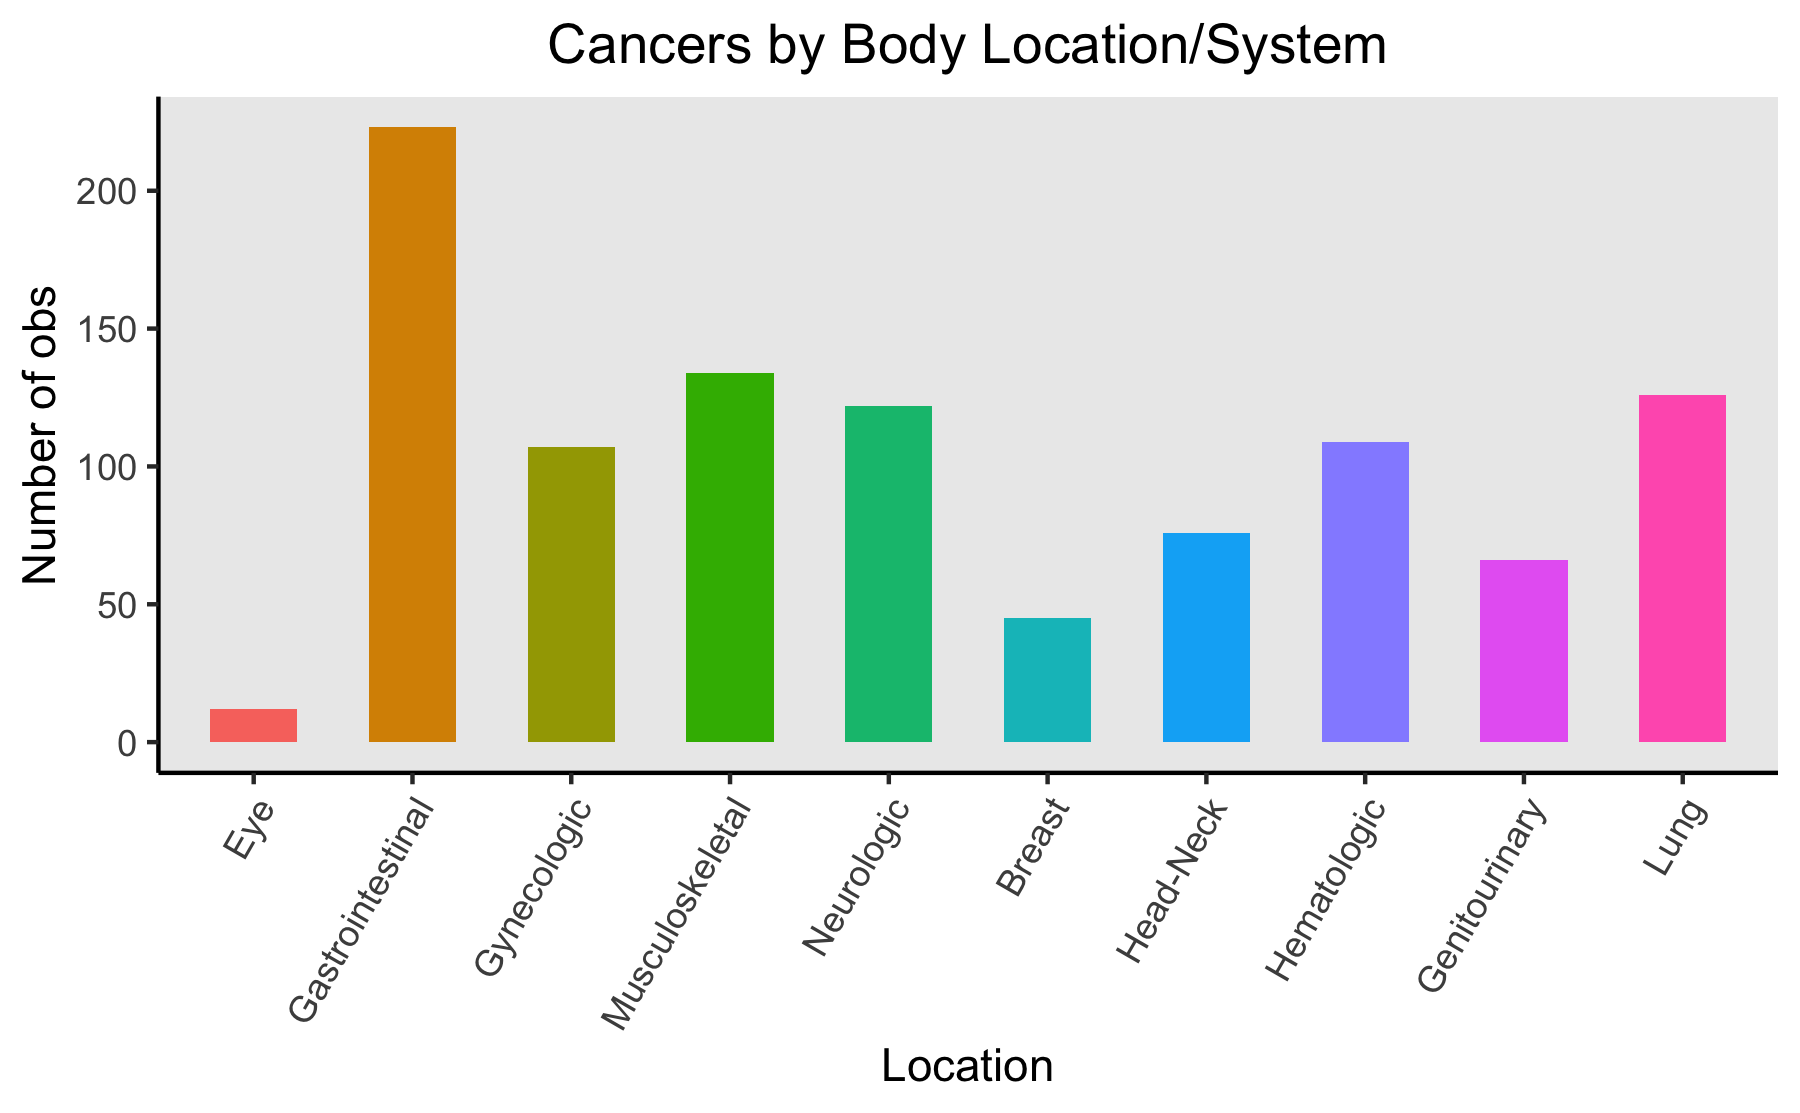
\includegraphics[width=0.65\textwidth]{plot1.png}
	\captionof{figure}{Cancer classes}\label{fig1}
\end{wrapfigure}
We grouped the various cancer types in 10 classes according to common medical knowledge\footnote{Cancer types grouped by body location: \url{https://www.cancer.gov/types/by-body-location}} and we obtained classes as reported in Figure \ref{fig1}.  "Eye" was the smallest one as there were only $16$ observations, $5$ of which labelled as "Enginereed". On the other hand, "Gastrointestinal" was the largest group and it comprehended $7$ types of cancer,  making this group quite heterogeneous. \\
We investigated two Binary classification problems, Blood vs Rest and Lung vs Rest, and the Multiclass problem. We chose "Lung" because of the nature of such a class: it was the most numerous group composed only by Lung cancer samples. The choice of "Blood" was instead driven by some underlying biological knowledge: Blood cancer is quite different from other tumours because
\begin{itemize}
	\item Leukemia, Lymphom and Myeloma are the main kinds of cancer but they all affect white blood cells;
	\item blood is in the whole body, and so the cancer is, too,	
	%\item not all blood cancers require a treatment, just periodical monitoring.
\end{itemize} 

\section{Methods}
Let us briefly illustrate the algorithms we used. Our methodology was characterized by three steps:
\begin{enumerate}
	\item fit the model using all the features;
	\item identify the most important variables based on some measure of importance;
	\item use these genes to fit a reduced version of the classifier and find out its performance.
\end{enumerate}
Clearly, each procedure involved fitting a model twice: the all-features version and the reduced one. We were thus forced to split the dataset into two further chunks. This was crucial to ensure independence of the two models and remove any sort of correlation.

\subsection{Random Forest}
We started by fitting Random Forest (RF) models as they frequently performs well on imbalanced and correlated high-dimensional data. We used Variable Importance to identify the most relevant features. This measure is calculated in three steps. First, prediction accuracy are measured on the out-of-bag samples. Then, the values of the variable are randomly shuffled, keeping all other variables the same. Finally, the decrease in prediction accuracy on the shuffled data is measured and the mean decrease in accuracy across all trees is reported. 

\begin{wrapfigure}{l}{0.27\textwidth}
	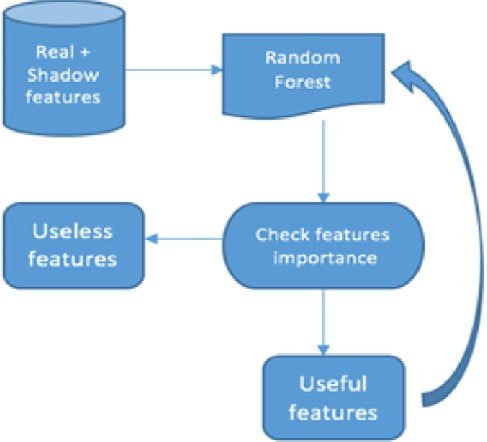
\includegraphics[width=0.27\textwidth]{Boruta-Algorithm.jpg}
	\captionof{figure}{Boruta algorithm}\label{fig2}
\end{wrapfigure}
Intuitively, the random shuffling means that, on average, the shuffled variable has no predictive power. \\
Hence, Variable Importance measures how much accuracy decreases because of removing a variable. Here, we used it in two different ways:
\begin{itemize}
	\item \textit{Cross-validation}: we performed a 5-fold Cross-validation on the model, averaged the importance values and selected the top most important features;
	\item \textit{Boruta algorithm}\footnote{Boruta algorithm: \url{https://www.researchgate.net/publication/220443685_Boruta_-_A_System_for_Feature_Selection}}: Boruta repeatedly measured feature importance and then performed statistical tests to screen out irrelevant features. Simple scheme is drawn in Figure \ref{fig2}. % The procedure terminates when all features are either decisively relevant or decisively irrelevant. Simple scheme is drawn in Figure \ref{fig2}. 
\end{itemize} 

\subsection{SVM-Lasso}
Support vector machines (SVM) are based on the idea of finding a hyperplane that best separate classes. Here, we combined this method with the classical Lasso penalty, so that the objective function to be minimized was:
\begin{equation*}
\dfrac{1}{n} \sum_{i=1}^n hingeLoss(y_i(x_i w + t)) + \lambda ||w||_1  \qquad	\text{where} \qquad  hingeLoss(z) = max\{0, 1-z\}
\end{equation*}
The parameter $\lambda$ has been chosen via cross-validation. Thanks to Lasso penalty, we obtained sparsity in predictors: some $w_i$ were shrunken all the way to zero, whereas the others identified important features. 

\subsection{Neural Networks}
Neural Networks (NN) are efficient models to capture non-linear relationships between predictors and target variables. In this context, we trained NN with two hidden layers of width $400/500$ and $300$ respectively and we chose \textit{ReLU} as activation function for the hidden layer, \textit{sigmoid} and \textit{softmax} for the output layer of, respectively, binary and multiclass classifications. \\
Given that the binary problems were a little unbalanced, we tried both the usual \textit{Cross Entropy} loss function and the \textit{Focal Loss}, defined as 
\begin{equation*}
FL(z) = \alpha \cdot (1 - z)^{\gamma} \log{z} \text{,  \hspace{3pt} with }z \in [0,1]  \text{ and } \alpha,  \gamma \geq 0
\end{equation*}
Note that \textit{Focal Loss} can be extended for dealing with multiclass classification tasks\footnote{Focal Loss: \url{https://arxiv.org/pdf/1708.02002.pdf}}. \\
Once our NNs were fitted,  we ranked variables according to the Olden Importance measure\footnote{Olden Importance: \url{https://depts.washington.edu/oldenlab/wordpress/wp-content/uploads/2013/03/EcologicalModelling_2004.pdf}}, selected the first ones and trained a reduced version of the classifier on them. We used Olden's importance as it can work with multiple hidden layers and multiclass problems. 

\section{Results}
\subsection{Binary classifications}
%PCA
Before starting our Binary classifications on Blood and Lung cancer, we ran a Principal Component Analysis to gain some valuable insights. We noticed a surprising result: even if observations formed a cloud of points, Blood cancer cells were mainly concentrated in just one part of the 3-dimensional plot. The same did not happen for Lung cancer observations.

\subsubsection{Random Forests}
%We then moved to RF classifiers.
Unfortunately, we could not build a proper model for Lung vs Rest. Even after a tuning on tree parameters, our RF was not able to detected the minority class. Thanks to SMOTE, we adjusted the frequency of those observations from $11\%$ to $50\%$ and the refitted RF gave us a slightly better result: at least one third of Lung cancer cells was correctly predicted. We also focused on pruning subtrees. In particular, we carried out a Randomized search and found an optimal complexity parameter for the Minimal Cost-Complexity Pruning. However, this new RF classifier had reached the same accuracy of before. We reported the respective average recall in Table \ref{table:big_models}. \\
Since all our models were not good enough in classifying Lung cancer, we retained that selecting the most important features was pointless and incorrect in terms of real applications. \\
On the other hand, we obtained great results in Blood vs Rest classification. Even though Blood cancer observations were only the $11\%$ of the total, we did not need any adjustments for the minority class. Indeed, thanks to proper tuning on trees parameters and a correction on class weights, we reached $98\%$ of mean accuracy. For completeness, we fitted also a RF with Cost-Complexity Pruning and we find the same accuracy. \\
Then, we removed unnecessary features by performing a 5-fold Cross-validation. Thanks to Variable Importance values, we could indeed selected the most relevant genes for each of the 5 models. As more rigorous way to pursue variable selection, we applied Boruta algorithm, too. As shown in Table \ref{table:selected variables}, Boruta individuated a higher number of important features than our manual method and, in particular, they agreed only on $84$ genes. As mentioned above, we fitted a RF on a new reduced dataset, where cancer instances accounted by $9\%$ of the total. Besides weighting classes, no further parameters were specified and, nevertheless, this RF classifier predicted correctly $6$ tumour cells out of $7$.   


\subsubsection{SVM-Lasso}
%Let us explore our SVM models.


\subsubsection{Neural Networks}
After several trials and different tuning, we obtained the best NN for the Lung vs Rest classification by using the \textit{Focal Loss} function. Here, we balanced our dataset by means of the Random Under Sampler but we did not reach the accuracy we hoped for. In fact, two third of Lung cancer instances were correctly classified but at the cost of getting many false positive predictions. Hence, we did not select the most important features for the same motivations as before. 
Not surprisingly, NN classifier for Blood vs Rest provided an excellent performance. After balancing again our dataset, we build the model with only two hidden layers and \textit{Cross Entropy} loss function. Then, all Blood cancer instances were classified rightly and almost none misclassification error occurred. \\
Furthermore, we selected the most important genes ranked according to Olden's importance. Since NN are especially suitable in handling high-dimensional data, decided to keep more features than RF and try the simplest NN model, i.e. built as a "vanilla" neural net (one single hidden layer). As result, we reached an accuracy of $98.8\%$, classifying correctly all Blood cancer cells.







\begin{table}[h!]
	\caption{Average recall of the models fitted with all the features}
	\centering
	\begin{tabular}{c c c}
		\hline\hline
		Task & RF & NN \\ [0.5ex] % inserts table %heading
		\hline
		Blood & 0.977  & 0.986 \\
		Lung & 0.649  & 0.632 \\
		Multiclass & --- & --- \\ [1ex]
		\hline
	\end{tabular}
	\label{table:big_models}
\end{table}

\begin{table}[h!]
	\caption{Selected variables}
	\centering
	\begin{tabular}{c c c c c}
		\hline\hline
		Task & RF & Boruta & SVM-Lasso & NN \\ [0.5ex] % inserts table %heading
		\hline
		Blood & 109 & 118 & 108 & 300 \\
		Multiclass & --- &  --- & --- & --- \\ [1ex]
		\hline
	\end{tabular}
	\label{table:selected variables}
\end{table}

\begin{table}[h!]
	\caption{Average recall of reduced models}
	\centering
	\begin{tabular}{c c c c}
		\hline\hline
		Task & RF & SVM-Lasso & NN \\ [0.5ex] % inserts table %heading
		\hline
		Blood & 0.929 & --- & 0.993 \\
		Multiclass & --- &  --- & --- \\ [1ex]
		\hline
	\end{tabular}
	\label{table:reduced_models}
\end{table}





\subsection{Multiclass classification}
When working with the multiclass problem we decided to remove the group "Eye" because it was a small heterogeneous group that even after tuning for RF and NN held the worst accuracy scores. "Eye" was a cluster of different types of cancer: this didn't create problems when we were using a One vs All aproach but with multiclass the effects of doing the cluster ourselves was mor evident.  
So after removing the group "Eye", we did the same as before and split the dataset in two.

\subsubsection{Random Forests}
We considered two different random forests, the first with the same parametes as the one used in Blood vs All random forest. Looking at the confusion matrix we can see hat most of the missclassification errors are data points classified as Gastrointestinal. Gastrointestinal was the biggest cluster we consider with a lot of different cancers so the genes( i.e. the features) important can be different within the cluster. To limit the weight of Gastrointestinal we decided to tune by hand the class weights. In this way we solve two problems: we reduced the importance of the group Gastrointestinal and we achieved at least one correct classification in each class. At this point we used cross validation to select five models and we extracted the most important features by looking at their relative importance in every model subjected to their presence in every model. We set a threshold to obtain  $(\sim   1700)$ features and with this we created a reduced model that we fitted using the validation set we had created at the beginning.


\subsubsection{SVM-Lasso}

\subsubsection{Neural Networks}
We first fitted a toy NN with only one hidden layer to see how the net worked.
We then fitted three different NN: the first increasing by one the number of hidden layers, the second changing the loss function with the Focal loss and the third using again the Focal loss, but changing the alpha parameter w.r.t. the class percentage in the set.
The three models held similar result with the second one being slightly more accurate. Once this NNs were fitted, we ranked the variable according to the Olden Importance measure, selected the first 1700 and used them to construct a reduced version of the classifier on the validation set.
The increment in the number of feature used for fitting the reduced model w.r.t. the binary NN model was beacuse we are now trying to separate nine different classes so we need much more information than before.


\section{Conclusion and future works}
\begin{itemize}
	\item reiterate key findings
	\item limitations: data high correlated,  no medical knowledge,  no meaning at selected genes
	\item suggest for the future: work with a med student,  try other classes or methods,  improve lung in some way
\end{itemize}

We approached the multiclass problem using three different techniques: RF, NN, SVM-Lasso and all three methods gave us good results. We can't say the same for the reduced models: while NN maintain an overall good performance using the same models, the RF need to be retuned to reach a similar performance. 


\end{document}